\section{Retrieval Augmented Generation (RAG)}

\subsection{Introduction}

Large language models (LLMs) have demonstrated significant success, yet they continue to encounter substantial limitations, particularly in tasks that are domain-specific or knowledge-intensive \cite{kandpal2023large}. A prominent issue is the generation of "hallucinations" \cite{zhang2023sirens}, where LLMs produce responses to queries that exceed their training data or necessitate up-to-date information. To mitigate these challenges, Retrieval-Augmented Generation (RAG) improves LLM performance by retrieving pertinent document chunks from an external knowledge base through semantic similarity calculations. By incorporating external knowledge, RAG substantially reduces the likelihood of generating factually incorrect content. The integration of RAG into LLMs has become widespread, establishing it as a crucial technology for advancing chatbots and enhancing the practical applicability of LLMs in real-world scenarios.

To address the limitations of generative AI, researchers and engineers have developed innovative methods, including the Retrieval-Augmented Generation (RAG) approach. RAG gained significant attention among generative AI developers following the release of the seminal paper "Retrieval-Augmented Generation for Knowledge-Intensive NLP Tasks" by Lewis et al. (2020) at Facebook AI Research  \cite{lewis2021retrievalaugmented}. RAG enhances the quality and relevance of generated text by combining the strengths of generative AI with retrieval techniques. Unlike traditional generative models that depend solely on their internal knowledge, RAG incorporates an additional step of retrieving information from external sources, such as databases, documents, or the web, before generating a response. This integration enables RAG to access up-to-date information and context, making it especially valuable for applications requiring accurate and current information.

RAG technology has seen rapid development in recent years, as illustrated by the technology tree summarizing related research in Figure \ref{fig:rag-tree}. The evolution of RAG within the era of large models can be divided into several distinct stages. Initially, the inception of RAG coincided with the rise of the Transformer architecture, focusing on improving language models by integrating additional knowledge through Pre-Training Models (PTM). This early phase was marked by foundational efforts to refine pre-training techniques \cite{arora2023garmeetsrag}-\cite{borgeaud2022improving}. The subsequent emergence of ChatGPT \cite{ouyang2022training} represented a pivotal moment, showcasing powerful in-context learning (ICL) capabilities. Following this, RAG research shifted towards enhancing LLMs' ability to address more complex and knowledge-intensive tasks during the inference stage, spurring rapid advancements in RAG studies. Over time, the focus expanded beyond the inference stage to include fine-tuning techniques for LLMs, further enhancing RAG's capabilities.

\begin{figure}[H]
    \centering
    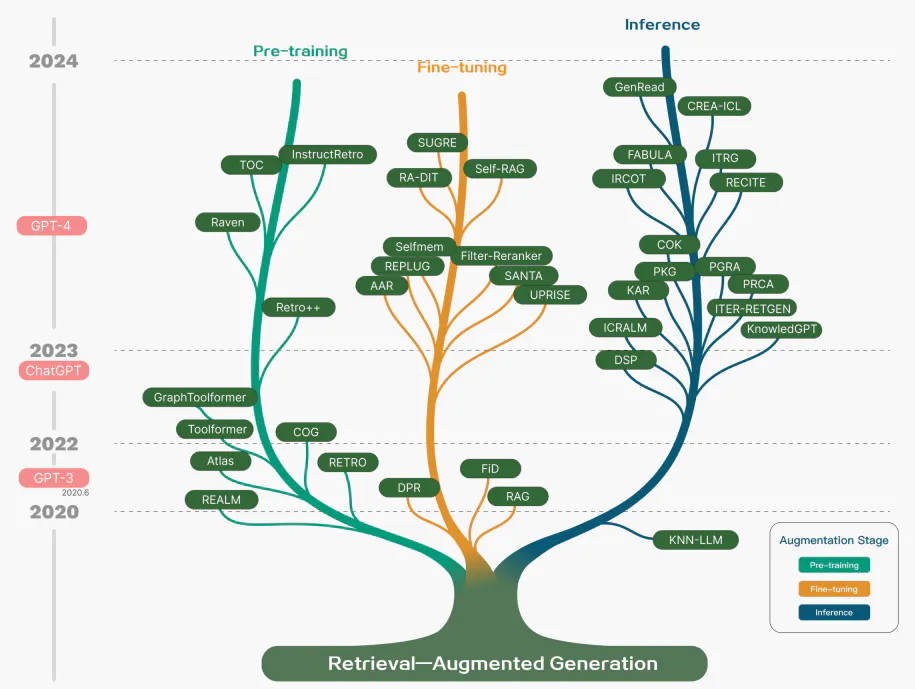
\includegraphics[width=\textwidth]{rag-tree.png}
    \caption{
        \it{ Technology tree of RAG research \cite{gao2024retrievalaugmented}}
    }
    \label{fig:rag-tree}
\end{figure}